\documentclass[../DoAn.tex]{subfiles}
\begin{document}

\section{Thiết kế kiến trúc}
\subsection{Lựa chọn kiến trúc phần mềm}
ĐATN này được xây dựng trên kiến trúc client-server. 
Đây là một kiến trúc được sử dụng rộng rãi cho các ứng dụng web, app mobile.

\textbf{Client}: Máy khách gửi yêu cầu tới máy chủ, nhận phản hồi và hiển thị 
dữ liệu nhận được ra cho người dùng.
\textbf{Server}: Máy chủ nhận yêu cầu từ client, xử lý và trả về dữ liệu cho máy khách.
\textbf{Database}: Lưu trữ dữ liệu và cung cấp dữ liệu cho máy chủ.
\begin{figure}[H]
    \centering
    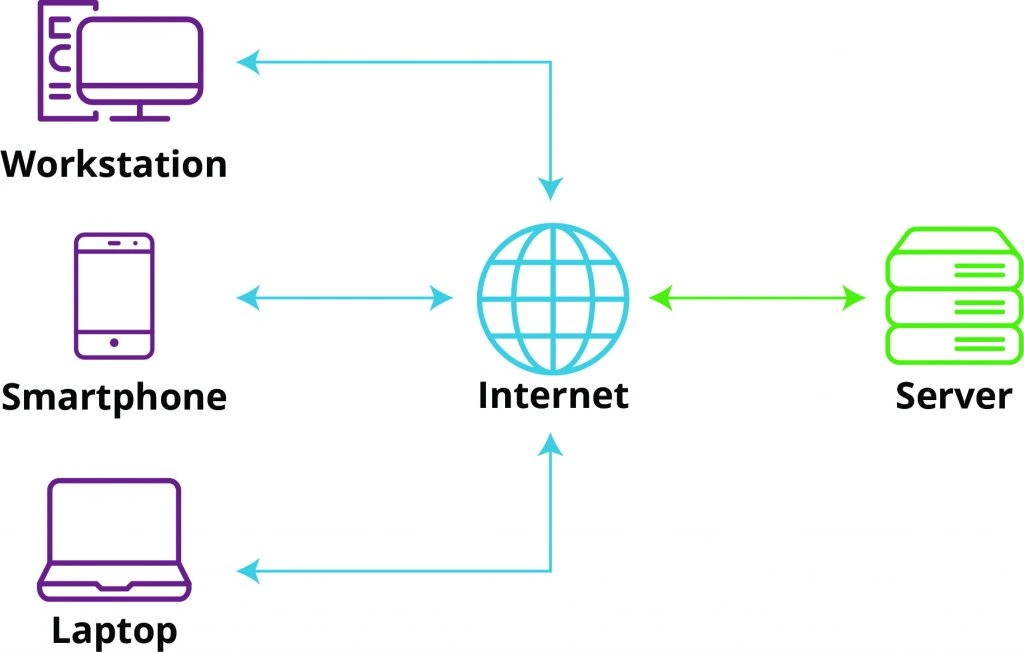
\includegraphics[width=0.8\textwidth]{Hinhve/Kien-truc-client-server.png}
    \caption{Kiến trúc client-server}
    \label{fig:Kien-truc-client-server}
\end{figure}

MVC (Model-View-Controller) là một mô hình kiến trúc phần mềm được sử dụng 
rộng rãi trong các ứng dụng web và app mobile.
MVC được sử dụng để tách biệt các thành phần của ứng dụng thành ba lớp chức năng riêng biệt:
\begin{itemize}
  \item \textbf{Model}: Lớp này chứa dữ liệu và logic xử lý dữ liệu.
  \item \textbf{View}: Lớp này hiển thị dữ liệu cho người dùng.
  \item \textbf{Controller}: Lớp này xử lý các yêu cầu từ người dùng và cập nhật 
  dữ liệu cho Model và View.
\end{itemize}

\begin{figure}[H]
    \centering
    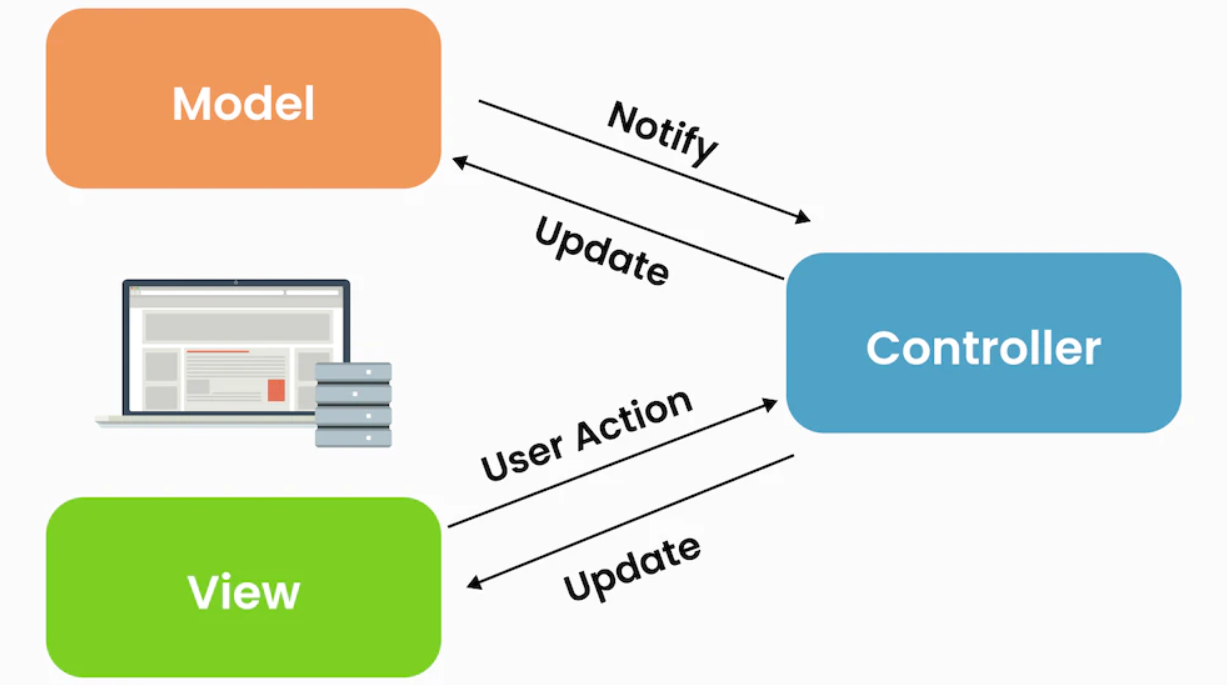
\includegraphics[width=0.8\textwidth]{Hinhve/Mo-hinh-mvc.png}
    \caption{Mô hình MVC}
    \label{fig:Mo-hinh-mvc}
\end{figure}

Mục đích của việc sử dụng kiến trúc MVC là để tách biệt các thành phần của 
ứng dụng thành ba lớp chức năng riêng biệt, giúp cho việc phát triển, bảo trì 
và mở rộng ứng dụng được dễ dàng hơn.
Một số ưu điểm của mô hình MVC:
\begin{itemize}
  \item Tổ chức mã nguồn tốt hơn: Giúp cho việc quản lý mã nguồn một cách dễ 
  dàng hơn, giảm thiểu sự phục thuộc giữa các thành phần.
  \item Tái sử dụng mã nguồn: Các thành phần có thể được sử dụng lại trong nhiều 
  ứng dụng khác nhau.
  \item Dễ dàng mở rộng: Dễ dàng thêm hoặc chỉnh sửa các chức năng mà không cần 
  phải thay đổi các thành phần khác.
\end{itemize}

Trong ứng dụng này, phía client gồm các thành phần chính như sau:
\begin{itemize}
    \item screens: Gồm các màn hình chính được sử dụng trong ứng dụng như: login\_screen, home\_screen, profile\_screen...
    \item service: Chứa các logic xử lý của ứng dụng.
    \item utils: Chứa các hàm hỗ trợ cho ứng dụng.
    \item widget: Chứa các widget dùng chung trong các screen như: card, list\_item
    \item assets: Chứa các tài nguyên như hình ảnh, icon, ...
\end{itemize}

Về phía server, ứng dụng được xây dựng trên framework NestJS, gồm các 
thành phần chính như sau:
\begin{itemize}
    \item module: nhóm các chức năng chính của ứng dụng như controller, service, dto... 
    \item controller: Nhận, xử lý yêu cầu và gửi phản hồi lại cho người dùng. 
    Đây là phần Controller trong mô hình MVC. 
    Máy khách chịu trách nhiệm là phần View trong mô hình MVC.
    Một số controller của ứng dụng như: travel.controller, user.controller, 
    driver.controller
    \item service: Chịu trách nhiệm xử lý các logic nghiệp vụ được sử dụng 
    bởi controller hoặc các service khác.
    \item middleware: Xử lý yêu cầu trước khi nó được gửi đến controller
\end{itemize}

\subsection{Thiết kế tổng quan}
\begin{figure}[H]
    \centering
    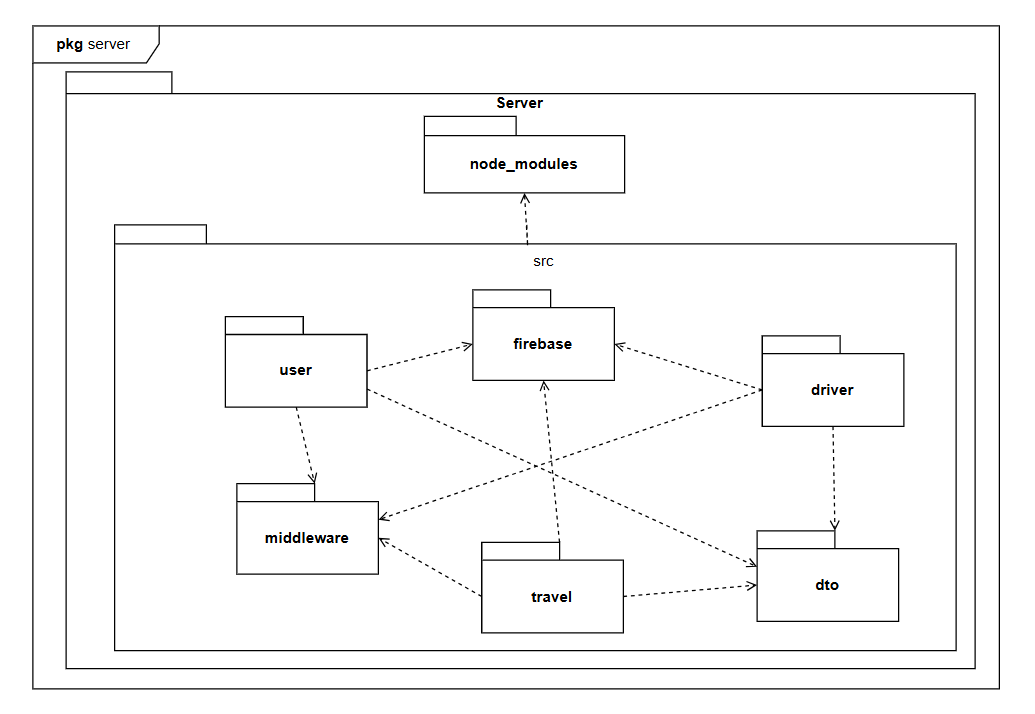
\includegraphics[width=0.8\textwidth]{Hinhve/Bieu_do_phu_thuoc_goi_server.png}
    \caption{Biểu đồ phụ thuộc gói Server}
    \label{fig:Bieu_do_phu_thuoc_goi_server}
\end{figure}

Hình \ref{fig:Bieu_do_phu_thuoc_goi_server} mô tả cấu trúc gói tổng thể phía server của hệ thống.
Tất cả các phụ thuộc được mô tả bằng mũi tên như trong hình.

Server bao gồm các gói sau:
\begin{itemize}
    \item node-modules: Chứa tất cả các module và thư viện mà server cần sử dụng.
    \item firebase: Định nghĩa các module, service giúp kết nối và tương tác với firebase.
    \item user: Quản lý người dùng của ứng dụng.
    \item driver: Quản lý tài xế của ứng dụng.
    \item travel: Quản lý các chuyến đi của người dùng.
    \item dto: Định nghĩa các đối tượng truyền dữ liệu.
    \item middleware: Xử lý các yêu cầu trước khi nó vào các controller tương ứng
\end{itemize}

\begin{figure}[H]
    \centering
    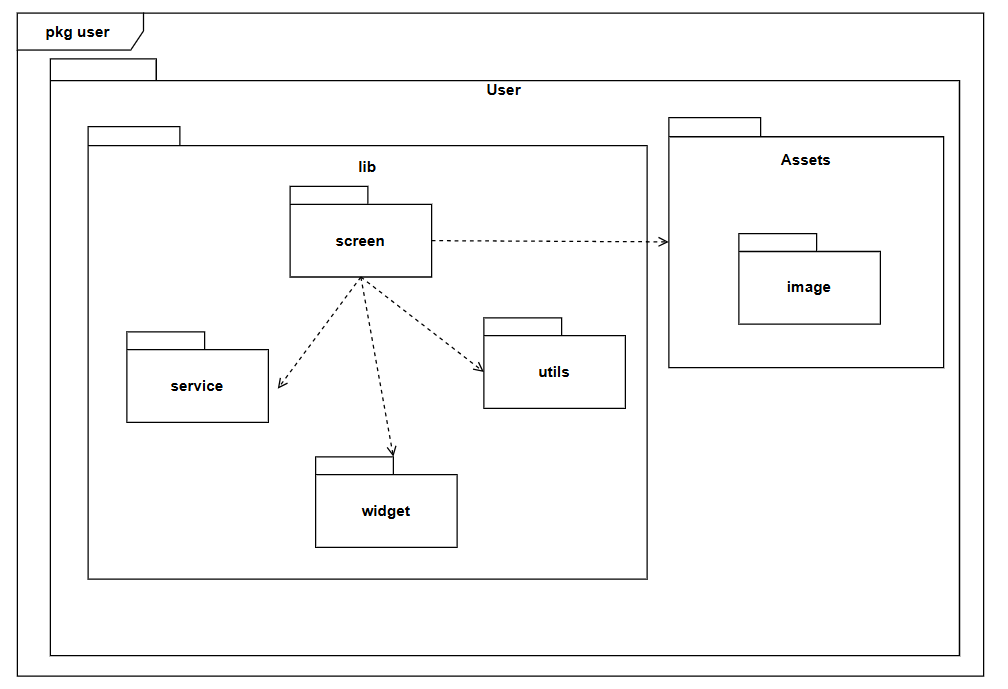
\includegraphics[width=0.8\textwidth]{Hinhve/Bieu_do_phu_thuoc_goi_user.png}
    \caption{Biểu đồ phụ thuộc gói Driver}
    \label{fig:Bieu_do_phu_thuoc_goi_user}
\end{figure}

Hình \ref{fig:Bieu_do_phu_thuoc_goi_user} mô tả cấu trúc gói phía user và driver của ứng dụng.
Tất cả các phụ thuộc được mô tả bằng mũi tên như trong hình.
\begin{itemize}
    \item assets: Chứa các tài nguyên như hình ảnh, icon, ...
    \item utils: Chứa các hàm hỗ trợ cho ứng dụng.
    \item widget: Chứa các widget dùng chung trong các screen như: loading, card...
    \item screens: Gồm các màn hình chính được sử dụng trong ứng dụng như: login\_screen, home\_screen, profile\_screen...
    \item service: Chứa các hàm xử lý logic của ứng dụng.
\end{itemize}

\subsection{Thiết kế chi tiết gói}
Sinh viên thiết kế và lần lượt vẽ biểu đồ thiết kế cho từng package, 
hoặc một nhóm các package liên quan để giải quyết một vấn đề gì đó. 
Khi vẽ thiết kế gói, sinh viên chỉ cần đưa tên lớp, không cần chỉ ra 
các thành viên phương thức và thuộc tính. SV tham khảo ví dụ minh họa 
trong Hình \ref{fig:Fig2}.

Sinh viên cần vẽ rõ ràng quan hệ giữa các lớp trong biểu đồ. Các quan 
hệ bao gồm: phụ thuộc (dependency), kết hợp (association), kết tập (aggregation), 
hợp thành (composition), kế thừa (inheritance), và thực thi (implementation). 
Các quan hệ này đều đã được minh họa trong \ref{fig:Fig2}.



\begin{figure}[H]
    \centering
    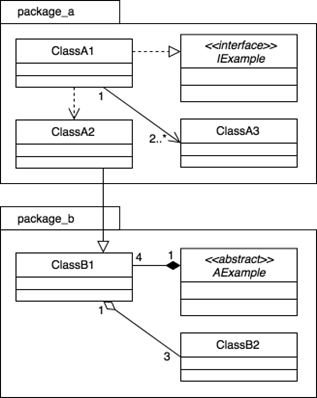
\includegraphics[width=0.8\textwidth]{Hinhve/Picture2.png}
    \caption{Ví dụ thiết kế gói}
    \label{fig:Fig2}
\end{figure}

\section{Thiết kế chi tiết}
\subsection{Thiết kế giao diện}

Giao diện của ứng dụng này được thiết kế để sử dụng trên điện thoại Android
Bố cục các thành phần trong các màn hình ứng dụng được thiết kế đơn giản
và dễ sử dụng. Người dùng có thể sử dụng ứng dụng mà không cần đọc bất 
kỳ hướng dẫn nào.

Thiết kế của ứng dụng cũng giảm thiểu việc sử dụng nhiều màu sắc khác nhau.
Thông thường, mỗi trang giao diện chỉ sử dụng 2-3 màu chính (đỏ, xanh lá, xanh dương) 
để tránh việc gây khó chịu đối với người dùng.
Ngoài ra việc sử dụng màu sắc cũng phản ánh tác dụng của chúng. Ví dụ: màu đỏ 
phản ánh việc xóa, hủy trong khi đó màu xanh lá phản ánh việc thêm mới, xác nhận.

Hầu hết màn hình có 3 phần chính gồm: phần tiêu đề ở trên cùng, phần nội dung ở giữa và phần điều hướng sang các màn khác ở dưới cùng.

\begin{figure}[H]
    \centering
    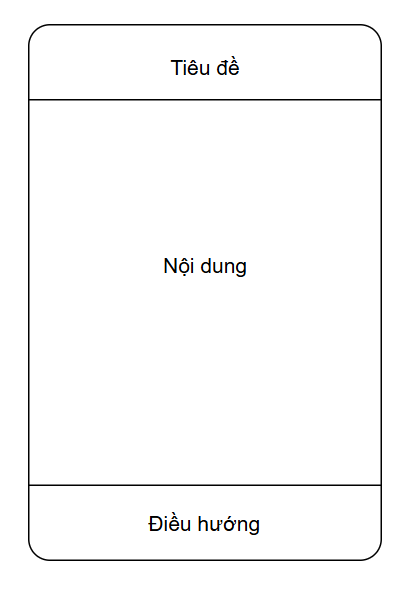
\includegraphics[width=0.8\textwidth]{Hinhve/Thiet_ke_man_hinh_chinh.png}
    \caption{Thiết kế chính các màn hình}
    \label{fig:Thiet_ke_chinh_ung_dung}
\end{figure}

Hình \ref{fig:Thiet_ke_chinh_ung_dung} mô tả thiết kế chính của các màn hình 
trong ứng dụng. Phần tiêu đề mô tả để biết đó đang là màn hình nào. 
Phần nội dung nằm ở giữa và chiếm phần lớn nhất. Phần điều hướng nằm ở dưới dùng chứa các nút 
để chuyển qua các màn hình khác.

Giao diện Đặt tài xế:
\begin{figure}[H]
    \centering
    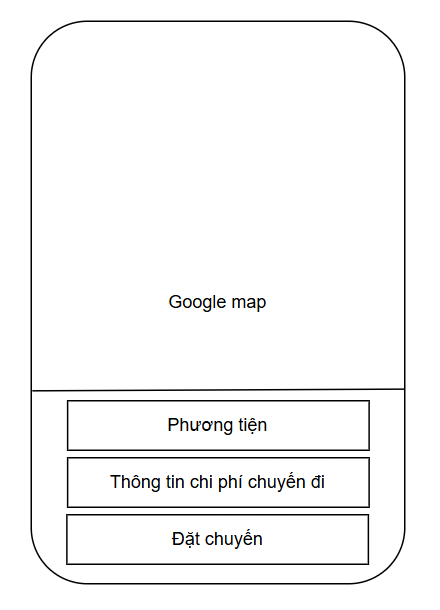
\includegraphics[width=0.8\textwidth]{Hinhve/Man_hinh_dat_tai_xe.png}
    \caption{Thiết kế màn hình Đặt tài xế}
    \label{fig:Thiet_ke_man_dat_tai_xe}
\end{figure}
Giao diện Thông tin người dùng:
\begin{figure}[H]
    \centering
    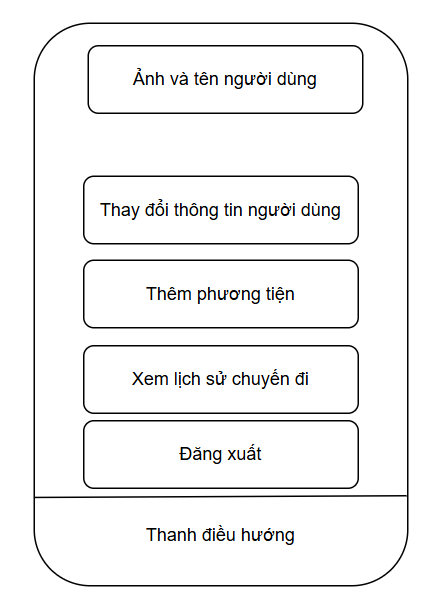
\includegraphics[width=0.8\textwidth]{Hinhve/Man_hinh_thong_tin_nguoi_dung.png}
    \caption{Thiết kế màn hình Thông tin người dùng}
    \label{fig:Man_hinh_thong_tin_nguoi_dung}
\end{figure}
Giao diện Lịch sử chuyến đi của người dùng:
\begin{figure}[H]
    \centering
    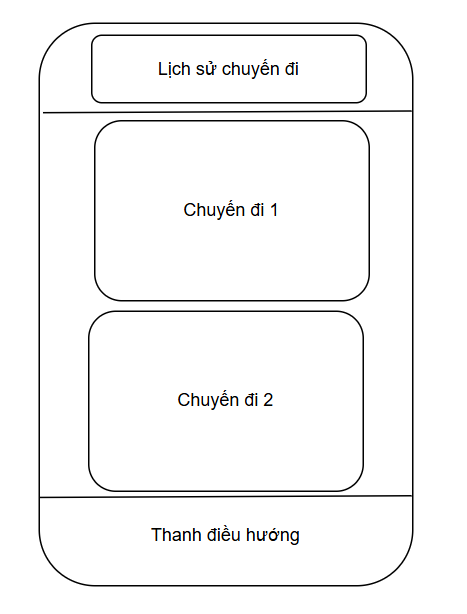
\includegraphics[width=0.8\textwidth]{Hinhve/Man_hinh_lich_su_chuyen_di_user.png}
    \caption{Thiết kế màn hình Lịch sử chuyến đi của người dùng}
    \label{fig:Thiet_ke_man_lich_su_chuyen_di_user}
\end{figure}

Giao diện Thông báo có chuyến đi mới của tài xế:
\begin{figure}[H]
    \centering
    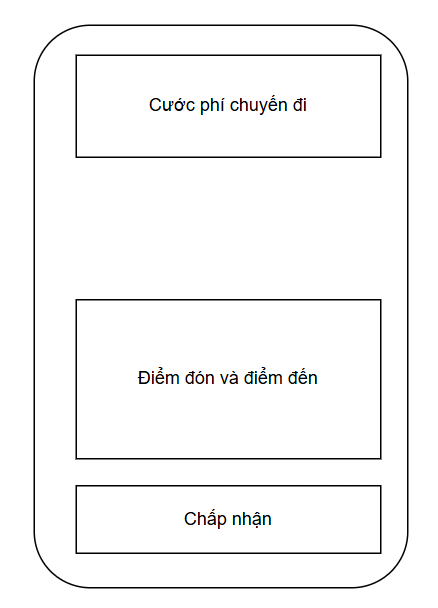
\includegraphics[width=0.8\textwidth]{Hinhve/Man_hinh_thong_bao_chuyen_di_driver.png}
    \caption{Thiết kế màn hình Thông báo có chuyến đi mới của tài xế}
    \label{fig:Man_hinh_thong_bao_chuyen_di_driver}
\end{figure}

\subsection{Thiết kế lớp}

\begin{figure}[H]
    \centering
    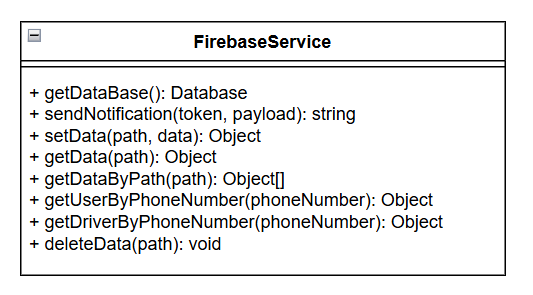
\includegraphics[width=0.8\textwidth]{Hinhve/Lop_firebase_service.png}
    \caption{Thiết kế lớp FirebaseService}
    \label{fig:Lop_firebase_service}
\end{figure}

Mô tả chi tiết các phương thức của lớp FirebaseService trong hình \ref{fig:Lop_firebase_service}:
\begin{itemize}
    \item getDatabase(): Lấy ra database hiện tại
    \item sendNotification(token, payload): Gửi thông báo bằng Firebase.
    \item setData(path, data): Thêm mới hoặc cập nhật dữ liệu.
    \item getData(path): Lấy dữ liệu theo đường dẫn.
    \item getDataByPath(path): Lấy dữ liệu theo đường dẫn và trả về mảng các đối tượng.
    \item getUserByPhoneNumber(phoneNumber): Lấy người dùng theo số điện thoại.
    \item getDriverByPhoneNumber(phoneNumber): Lấy tài xế theo số điện thoại.
    \item deleteData(path): Xóa dữ liệu khỏi database theo đường dẫn.
\end{itemize}

\begin{figure}[H]
    \centering
    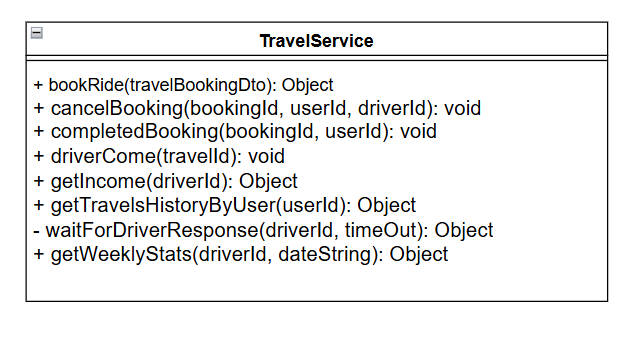
\includegraphics[width=0.8\textwidth]{Hinhve/Lop_travel_service.png}
    \caption{Thiết kế lớp TravelService}
    \label{fig:Lop_travel_service}
\end{figure}
Hình \ref{fig:Lop_travel_service} mô tả các phương thức của lớp TravelService gồm: 
\begin{itemize}
    \item bookRide(travelBookingDto): Tìm kiếm tài xế phù hợp, gửi thông báo cho tài xế rồi chờ phản hồi và gửi lại thông báo cho người dùng.
    \item cancelBooking(bookingId, userId, driverId): Hủy chuyến đi hiện tại.
    \item completedBooking(bookingId, userId): Hoàn thành chuyến đi hiện tại.
    \item driverCome(travelId): Thông báo là tài xế đã đến điểm đón.
    \item getIncome(driverId): Tính toán tổng thu nhập của tài xế trong 1 ngày.
    \item getTravelsHistoryByUser(userId): Lấy danh sách các chuyến đi của 1 người dùng.
    \item waitForDriverResponse(driverId, timeOut): Chờ phản hồi của tài xế về việc nhận chuyến đi.
    \item getWeeklyStats(driverId, dateString): Lấy tất cả các chuyến đi trong tuần hiện tại của tài xế.
\end{itemize}

\begin{figure}[H]
    \centering
    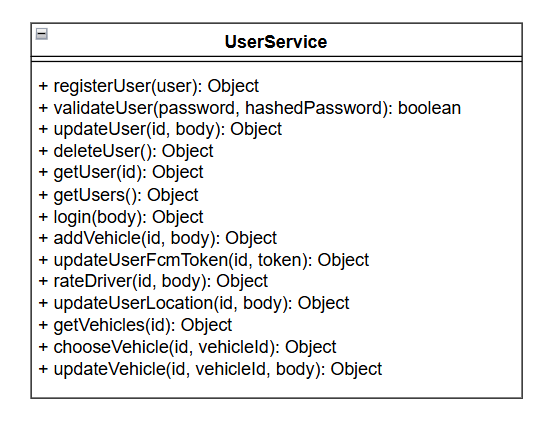
\includegraphics[width=0.8\textwidth]{Hinhve/Lop_user_service.png}
    \caption{Thiết kế lớp UserService}
    \label{fig:Lop_user_service}
\end{figure}
Mô tả chi tiết các phương thức có trong lớp UserService ở trong hình \ref{fig:Lop_user_service}:
\begin{itemize}
    \item registerUser(user): Thêm người dùng mới.
    \item validateUser(password, hashedPassword): Kiểm tra mật khẩu người dùng.
    \item updateUser(id, body): Cập nhật thông tin người dùng.
    \item deleteUser(id): Xóa người dùng ra khỏi database.
    \item getUser(id): Lấy thông tin người dùng.
    \item login(body): Đăng nhập vào ứng dụng.
    \item addVehicle(id, body): Thêm phương tiện cần lái hộ của người dùng.
    \item updateUserFcmToken(id, token): Cập nhật FCM token của người dùng.
    \item rateDriver(id, body): Đánh giá tài xế sau chuyến đi.
    \item updateUserLocation(id, body): Cập nhật vị trí của người dùng.
    \item getVehicles(id): Lấy các phương tiện của người dùng.
    \item chooseVehicle(id, vehicleId): Chọn phương tiện người dùng cần lái hộ.
    \item getVehicle(id): Lấy thông tin phương tiện mà người dùng đang cần lái hộ.
    \item updateVehicle(id, vehicleId, body): Cập nhật thông tin phương tiện của người dùng.
\end{itemize}

\begin{figure}[H]
    \centering
    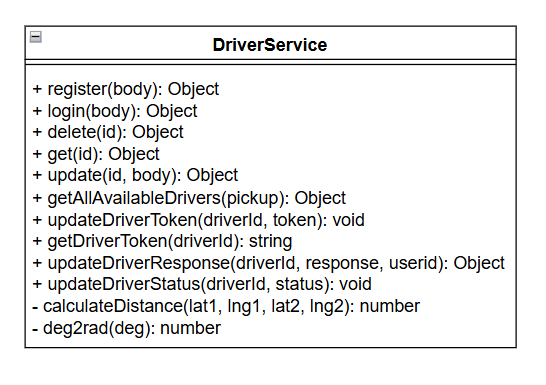
\includegraphics[width=0.8\textwidth]{Hinhve/Lop_driver_service.png}
    \caption{Thiết kế lớp DriverService}
    \label{fig:Lop_driver_service}
\end{figure}
Mô tả chi tiết các phương thức có trong lớp DriverService ở trong hình \ref{fig:Lop_driver_service}:
\begin{itemize}
    \item register(body): Đăng ký tài xế.
    \item login(body): Đăng nhập.
    \item delete(id): Xóa tài khoản.
    \item get(id): Lấy thông tin tài xế.
    \item update(id): Cập nhật thông tin tài xế.
    \item getAllAvailableDrivers(pickup): Lấy danh sách tài xế sẵn sàng nhận chuyến.
    \item updateDriverToken(driverId, token): Cập nhật FCM token của tài xế.
    \item getDriverToken(driverId): Lấy FCM token của người dùng.
    \item updateDriverResponse(driverId, response, userId): Cập nhật trạng thái đồng ý nhận chuyến của tài xế.
    \item updateDriverStatus(driverId, status): Cập nhật trạng thái sẵn sàng nhận chuyến của tài xế.
    \item calculateDistance(lat1, lng1, lat2, lng2): Tính khoảng cách giữa 2 địa điểm
    \item deg2rad(deg): Chuyển đổi từ số đo độ sang radian.
\end{itemize}

\subsection{Thiết kế cơ sở dữ liệu}
\begin{figure}[H]
    \centering
    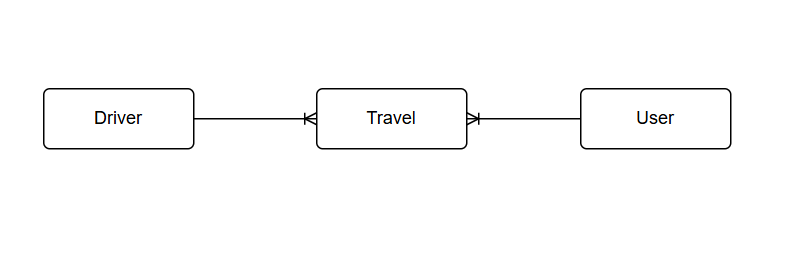
\includegraphics[width=0.8\textwidth]{Hinhve/Bieu_do_thuc_the_lien_ket.png}
    \caption{Biểu đồ thực thể liên kết}
    \label{fig:Bieu_do_thuc_the_lien_ket}
\end{figure}

\begin{table}[H]
    \centering
    \begin{tabular}{|l|l|}
    \hline
    \textbf{Thực thể} & \textbf{Giải thích}            \\ \hline
    User              & Lưu thông tin người dùng       \\ \hline
    Driver            & Lưu thông tin tài xế           \\ \hline
    Travel            & Lưu thông tin về các chuyến đi \\ \hline
    \end{tabular}
    \caption{Giải thích về các thực thể}
    \label{table:Bieu_do_thuc_the_lien_ket}
\end{table}

\begin{table}[H]
    \centering
    \begin{tabular}{|l|l|l|}
    \hline
    \textbf{Tên cột}           & \textbf{Loại dữ liệu} & \textbf{Ý nghĩa}                      \\ \hline
    avatar                     & String                & Ảnh đại diện của tài xế               \\ \hline
    avgRate                    & Number                & Đánh giá trung bình                   \\ \hline
    citizenIdentificationFront & String                & Ảnh mặt trước CCCD                    \\ \hline
    citizenIdentificationBack  & String                & Ảnh mặt sau CCCD                      \\ \hline
    drivingLicense             & String                & Ảnh giấy phép lái xe                  \\ \hline
    fcmToken                   & String                & FCM token nhận thông báo của Firebase \\ \hline
    fullName                   & String                & Họ tên đầy đủ                         \\ \hline
    location                   & Object                & Vị trí hiện tại của tài xế            \\ \hline
    password                   & String                & Mật khẩu                              \\ \hline
    phoneNumber                & String                & Số điện thoại                         \\ \hline
    rateDriver                 & Number[]              & Các đánh giá của người dùng           \\ \hline
    response                   & String                & Trạng thái đồng ý nhận cuốc           \\ \hline
    status                     & String                & Trạng thái hiện tại của tài xế        \\ \hline
    \end{tabular}
    \caption{Thiết kế chi tiết thực thể tài xế}
    \label{table:Thiết_kế_chi_tiết_thực_thể_tài_xế}
\end{table}

\begin{table}[H]
    \centering
    \begin{tabular}{|l|l|l|}
    \hline
    \textbf{Tên cột}    & \textbf{Loại dữ liệu} & \textbf{Ý nghĩa}                                      \\ \hline
    destinationLocation & Object                & Vị trí điểm đến                                       \\ \hline
    destinationString   & String                & Điểm đến                                              \\ \hline
    distance            & Number                & Khoảng cách                                           \\ \hline
    driverId            & String                & ID tài xế                                             \\ \hline
    duration            & Number                & Thời gian dự kiến khi không có phương tiện trên đường \\ \hline
    durationInTraffic   & Number                & Thời gian dự kiến khi có phương tiện trên đường       \\ \hline
    fare                & Number                & Giá cước                                              \\ \hline
    id                  & String                & Id chuyến đi                                          \\ \hline
    pickupLocation      & Number                & Vị trí điểm đón                                       \\ \hline
    pickupString        & String                & Điểm đón                                              \\ \hline
    poliline            & Object[]              & Đường đi đề xuất                                      \\ \hline
    status              & String                & Trạng thái chuyến đi                                  \\ \hline
    timeEnd             & String                & Thời gian kết thúc chuyến đi                          \\ \hline
    timeStart           & String                & Thời gian bắt đầu chuyến đi                           \\ \hline
    userId              & String                & ID người dùng                                         \\ \hline
    \end{tabular}
    \caption{Thiết kế chi tiết thực thể chuyến đi}
    \label{table:Thiết_kế_chi_tiết_thực_thể_chuyến_đi}
\end{table}

\begin{table}[H]
    \centering
    \begin{tabular}{|l|l|l|}
    \hline
    \textbf{Tên cột} & \textbf{Loại dữ liệu} & \textbf{Ý nghĩa}                         \\ \hline
    email            & String                & Email của người dùng                     \\ \hline
    fcmToken         & String                & FCM token để nhận thông báo của Firebase \\ \hline
    fullName         & String                & Họ tên của người dùng                    \\ \hline
    id               & String                & ID người dùng                            \\ \hline
    password         & String                & Mật khẩu                                 \\ \hline
    phoneNumber      & String                & Số điện thoại của người dùng             \\ \hline
    userAvatar       & String                & Ảnh đại diện của người dùng              \\ \hline
    userLocation     & Object                & Vị trí của người dùng                    \\ \hline
    vehicles         & Object[]              & Danh sách các phương tiện của người dùng \\ \hline
    \end{tabular}
    \caption{Thiết kế chi tiết thực thể người dùng}
    \label{table:Thiết_kế_chi_tiết_thực_thể_người_dùng}
\end{table}

\section{Xây dựng ứng dụng}
\subsection{Thư viện và công cụ sử dụng}

\begin{table}[H]
    \centering
    \begin{tabular}{|l|l|l|}
    \hline
    \textbf{Mục đích}  & \textbf{Công cụ}           & \textbf{Địa chỉ URL}                   \\ \hline
    IDE lập trình      & Visual Studio Code         & \url{https://code.visualstudio.com/}   \\ \hline
    Version Control    & Github                     & \url{https://github.com/}              \\ \hline
    Database           & Firebase Realtime Database & \url{https://firebase.google.com/}     \\ \hline
    Môi trường backend & NodeJS                     & \url{https://nodejs.org/en}            \\ \hline
    Framework backend  & NestJS                     & \url{https://nestjs.com/}              \\ \hline
    Ngôn ngữ frontend  & Dart                       & \url{https://dart.dev/}                \\ \hline
    Frameword fronend  & Flutter                    & \url{https://docs.flutter.dev/}        \\ \hline
    Lưu trữ files      & Firebase Storage           & \url{https://firebase.google.com/}     \\ \hline
    Tìm kiếm địa chỉ   & Google Map Platform        & \url{https://mapsplatform.google.com/} \\ \hline
    \end{tabular}
    \caption{Danh sách thư viện và công cụ sử dụng}
    \label{table:my_label}
\end{table}

\subsection{Kết quả đạt được}

Sau quá trình nghiên cứu, tìm hiểu và phát triển ứng dụng ViSafe BK, em đã triển khai bản APK phiên 
bản 1.0.0 chạy trên nền tảng Android. Ứng dụng có các chức năng chính như: tìm kiếm và đặt tài xế, xem thông tin về các chuyến đi.
Thông tin chi tiết về ứng dụng được trình bày trong bảng \ref{tab:thong_ke_thong_tin_ung_dung}:
\begin{table}[H]
    \centering
    \begin{tabular}{|l|l|l|}
    \hline
    \textbf{STT} & \textbf{Thông tin}                     & \textbf{Số liệu} \\ \hline
    1            & Số gói trong ứng dụng tài xế           & 4                \\ \hline
    2            & Số dòng code trong ứng dụng tài xế     & 2880             \\ \hline
    3            & Số file trong ứng dụng tài xế          & 20               \\ \hline
    4            & Số gói trong ứng dụng người dùng       & 4                \\ \hline
    5            & Số dòng code trong ứng dụng người dùng & 3370             \\ \hline
    6            & Số file trong ứng dụng người dùng      & 20               \\ \hline
    7            & Số gói trong ứng dụng backend          & 8                \\ \hline
    8            & Số dòng code trong ứng dụng backend    & 2570             \\ \hline
    9            & Số file trong ứng dụng backend         & 38               \\ \hline
    10           & Số document trong firebase             & 3                \\ \hline
    \end{tabular}
    \caption{Thống kê thông tin ứng dụng}
    \label{tab:thong_ke_thong_tin_ung_dung}
\end{table}
\subsection{Minh họa các chức năng chính}
Sau đây là màn hình các chức năng chính, quan trọng trong ứng dụng:

Giao diện màn hình Thông báo chuyến đi:
\begin{figure}[H]
    \centering
    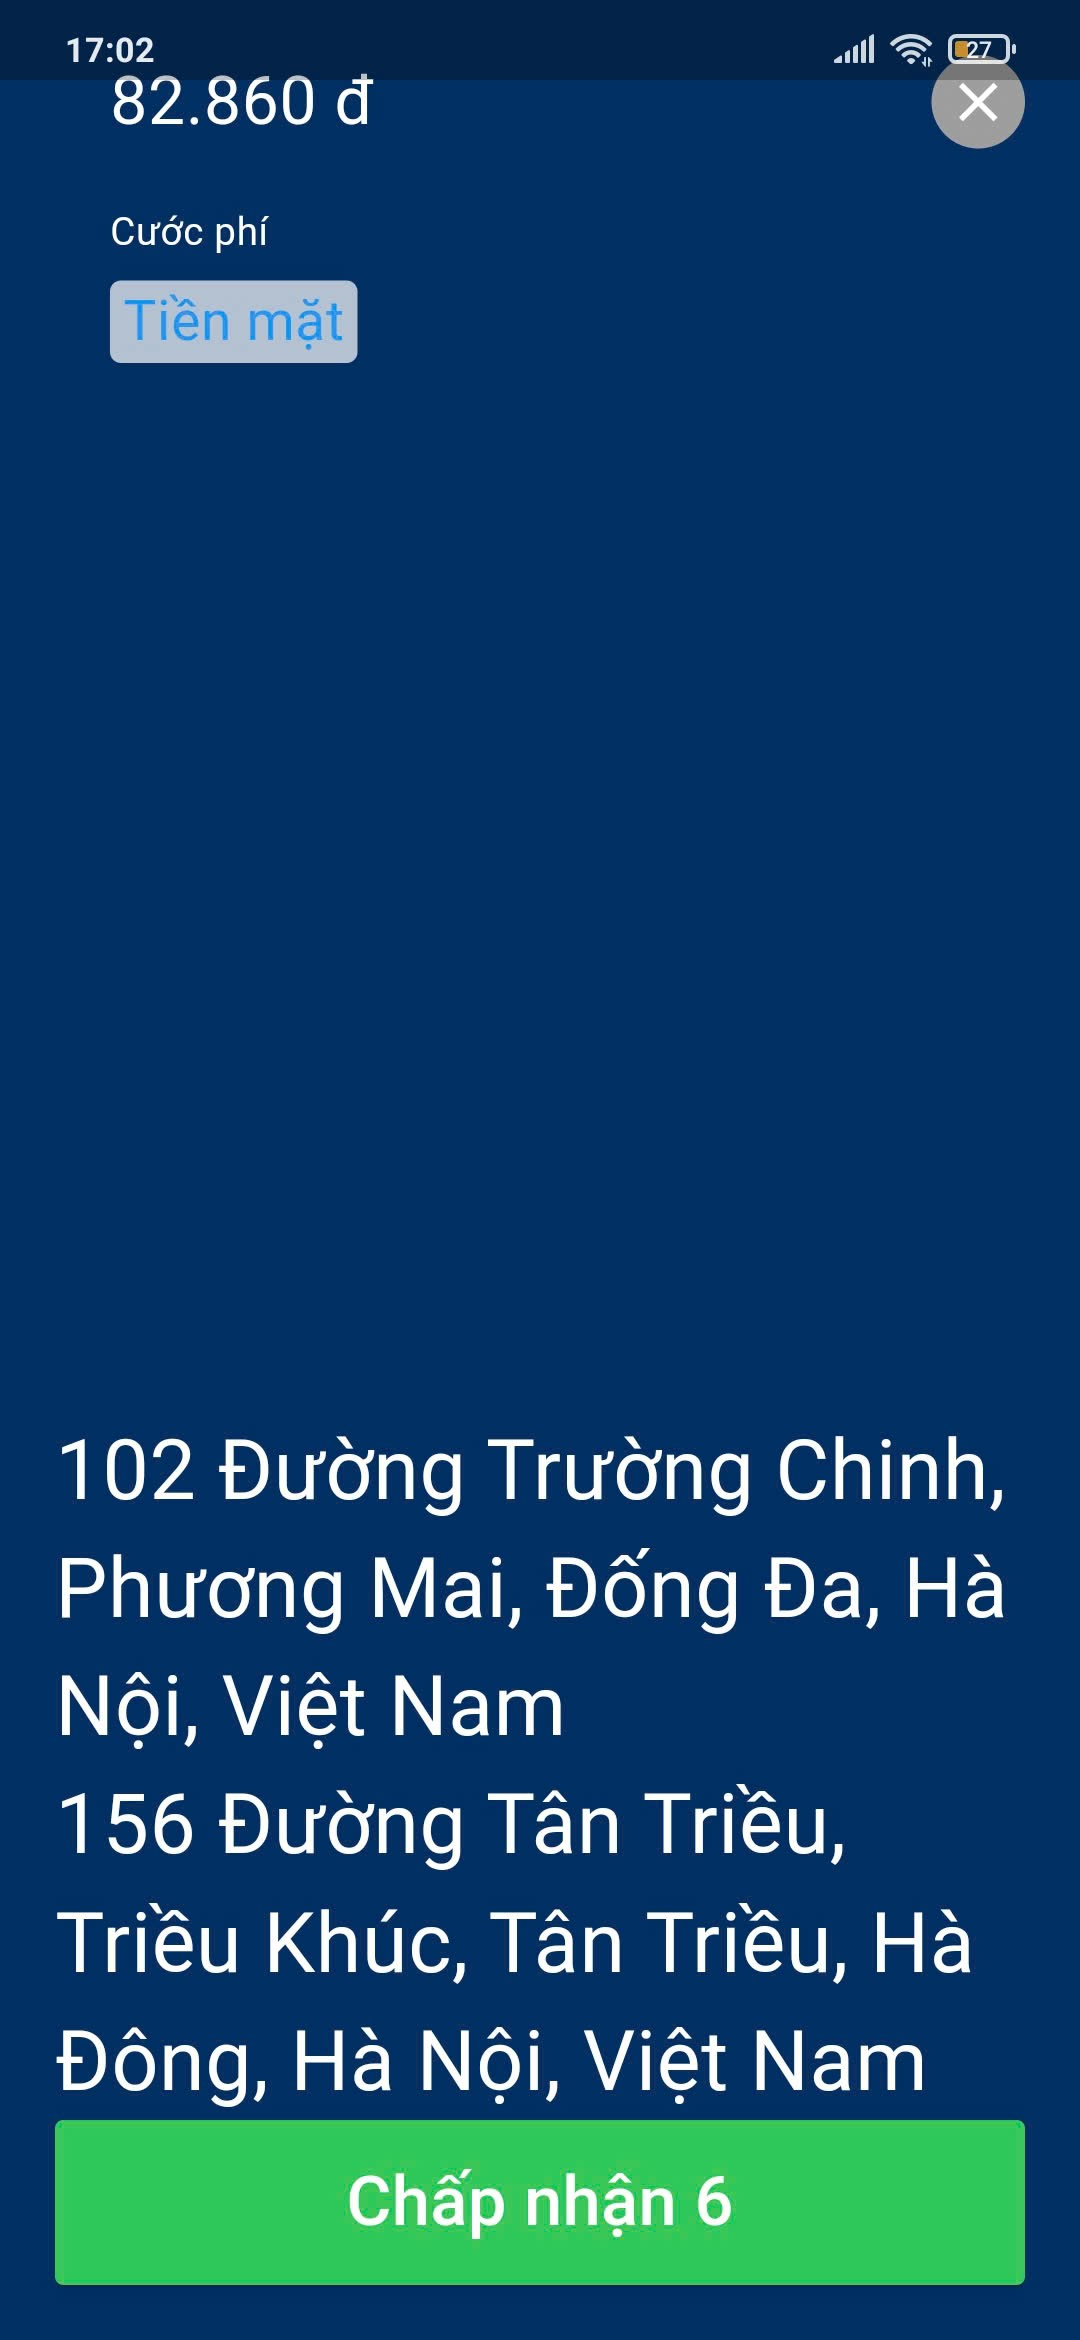
\includegraphics[width=0.8\textwidth]{Hinhve/Anh_man_hinh_thong_bao_chuyen_di.png}
    \caption{Màn hình thông báo chuyến đi của tài xế}
    \label{fig:Anh_man_hinh_thong_bao_chuyen_di}
\end{figure}
Màn hình thông báo chuyến đi cung cấp cho tài xế biết thông tin về giá của chuyến đi,
điểm đón và điểm đến.
Tài xế có 10 giây để quyết định chấp nhận hoặc không chấp nhận chuyến xe.

Giao diện màn hình Tìm đặt tài xế:
\begin{figure}[H]
    \centering
    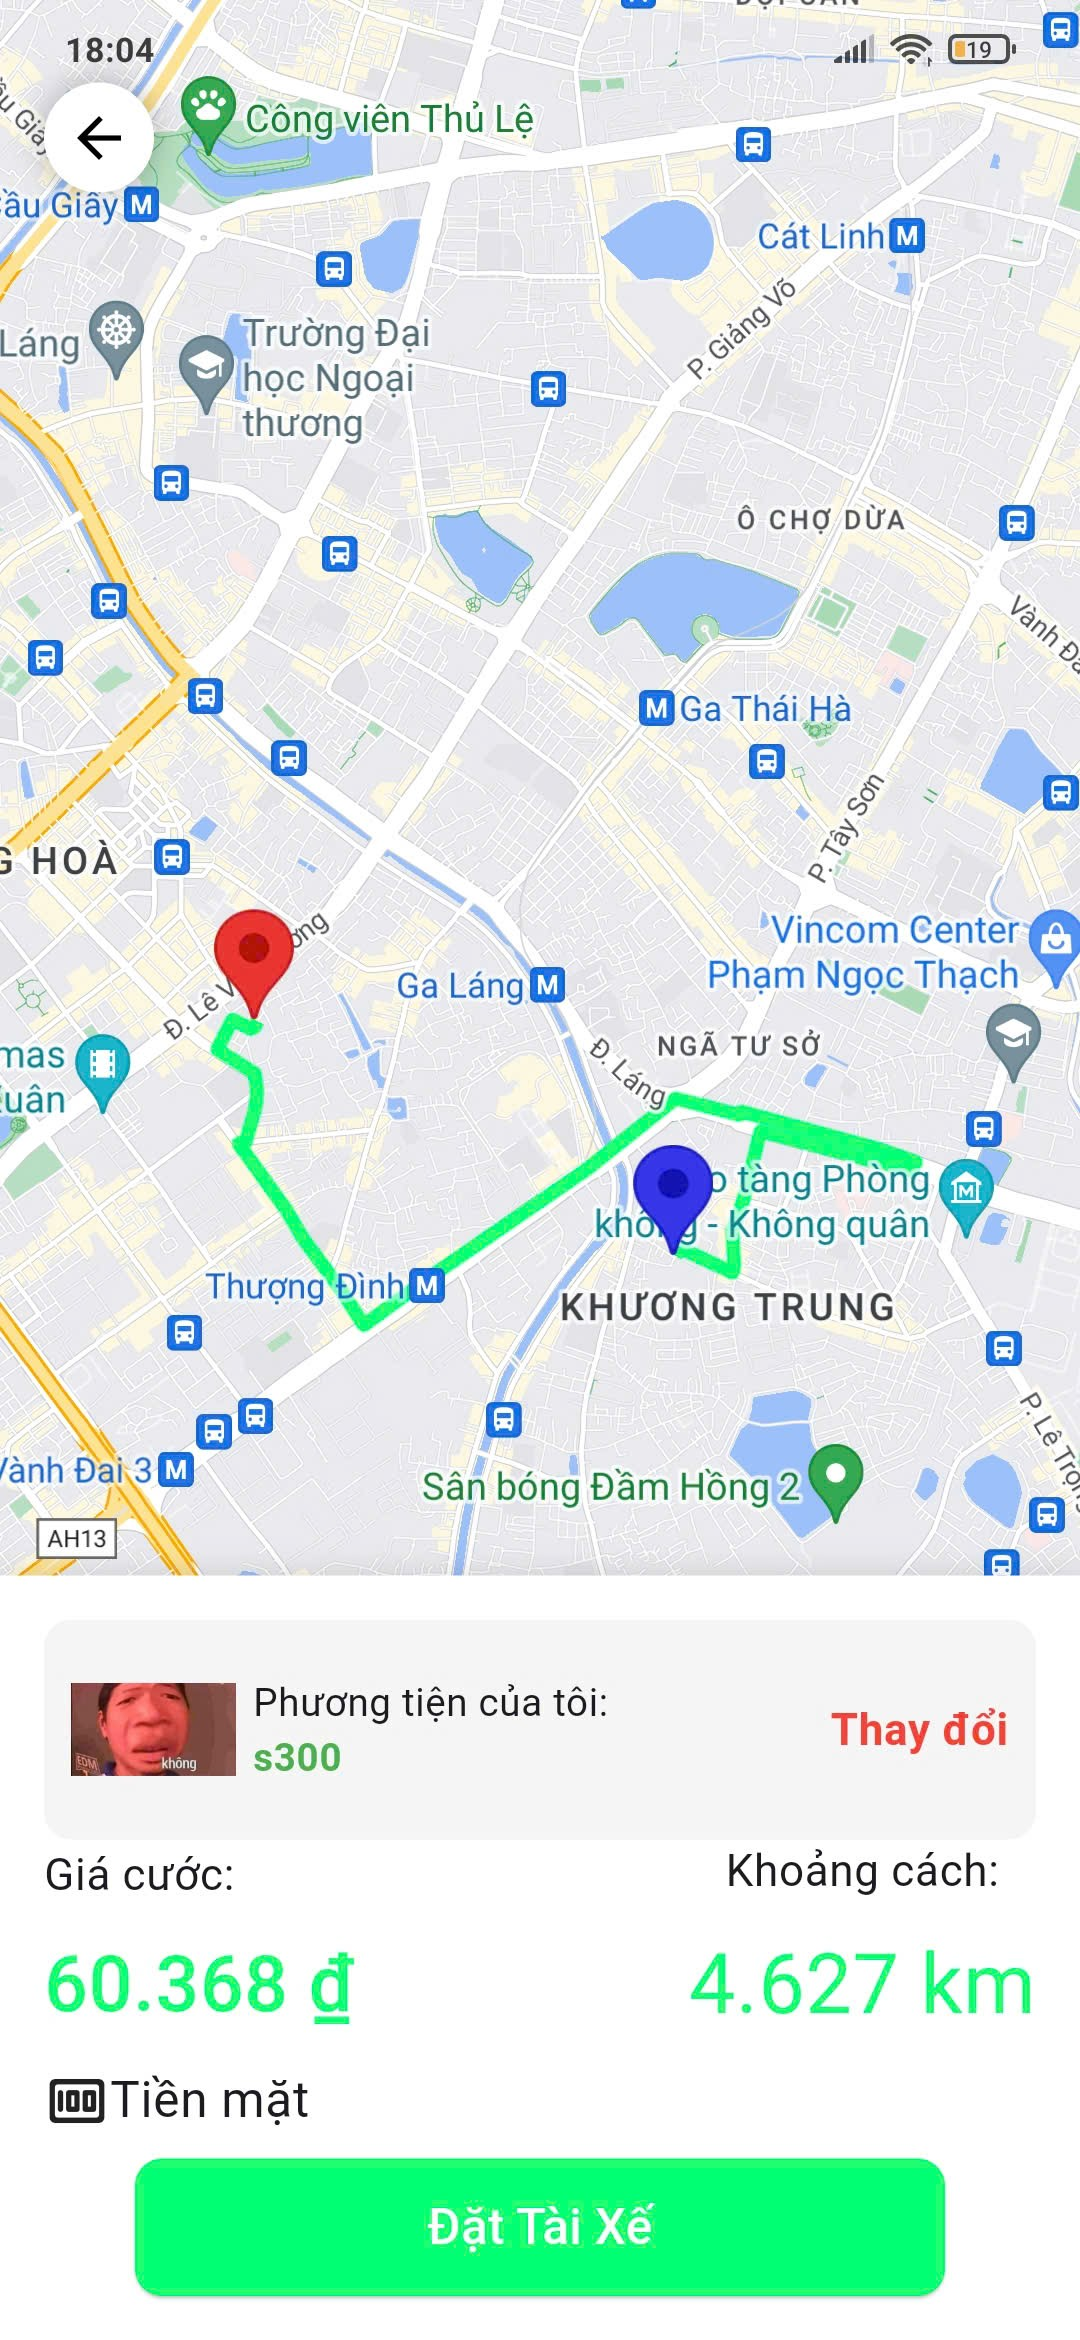
\includegraphics[width=0.8\textwidth]{Hinhve/Tim_dat_tai_xe.png}
    \caption{Màn hình Tìm đặt tài xế của người dùng}
    \label{fig:Tim_dat_tai_xe}
\end{figure}
Người dùng biết được chi phí phải trả cho chuyến đi, khoảng cách, tuyến đường đi dự kiến giữa 2 địa điểm.
Ngoài ra người dùng phải chọn phương tiện cần lái hộ trước khi đặt tài xế.
Sau khi có đầy đủ thông tin, người dùng nhấn "Đặt tài xế" để tìm tài xế thích hợp khi 
có nhu cầu thuê lái hộ.

Giao diện màn hình Lịch sử chuyến đi của người dùng:
\begin{figure}[H]
    \centering
    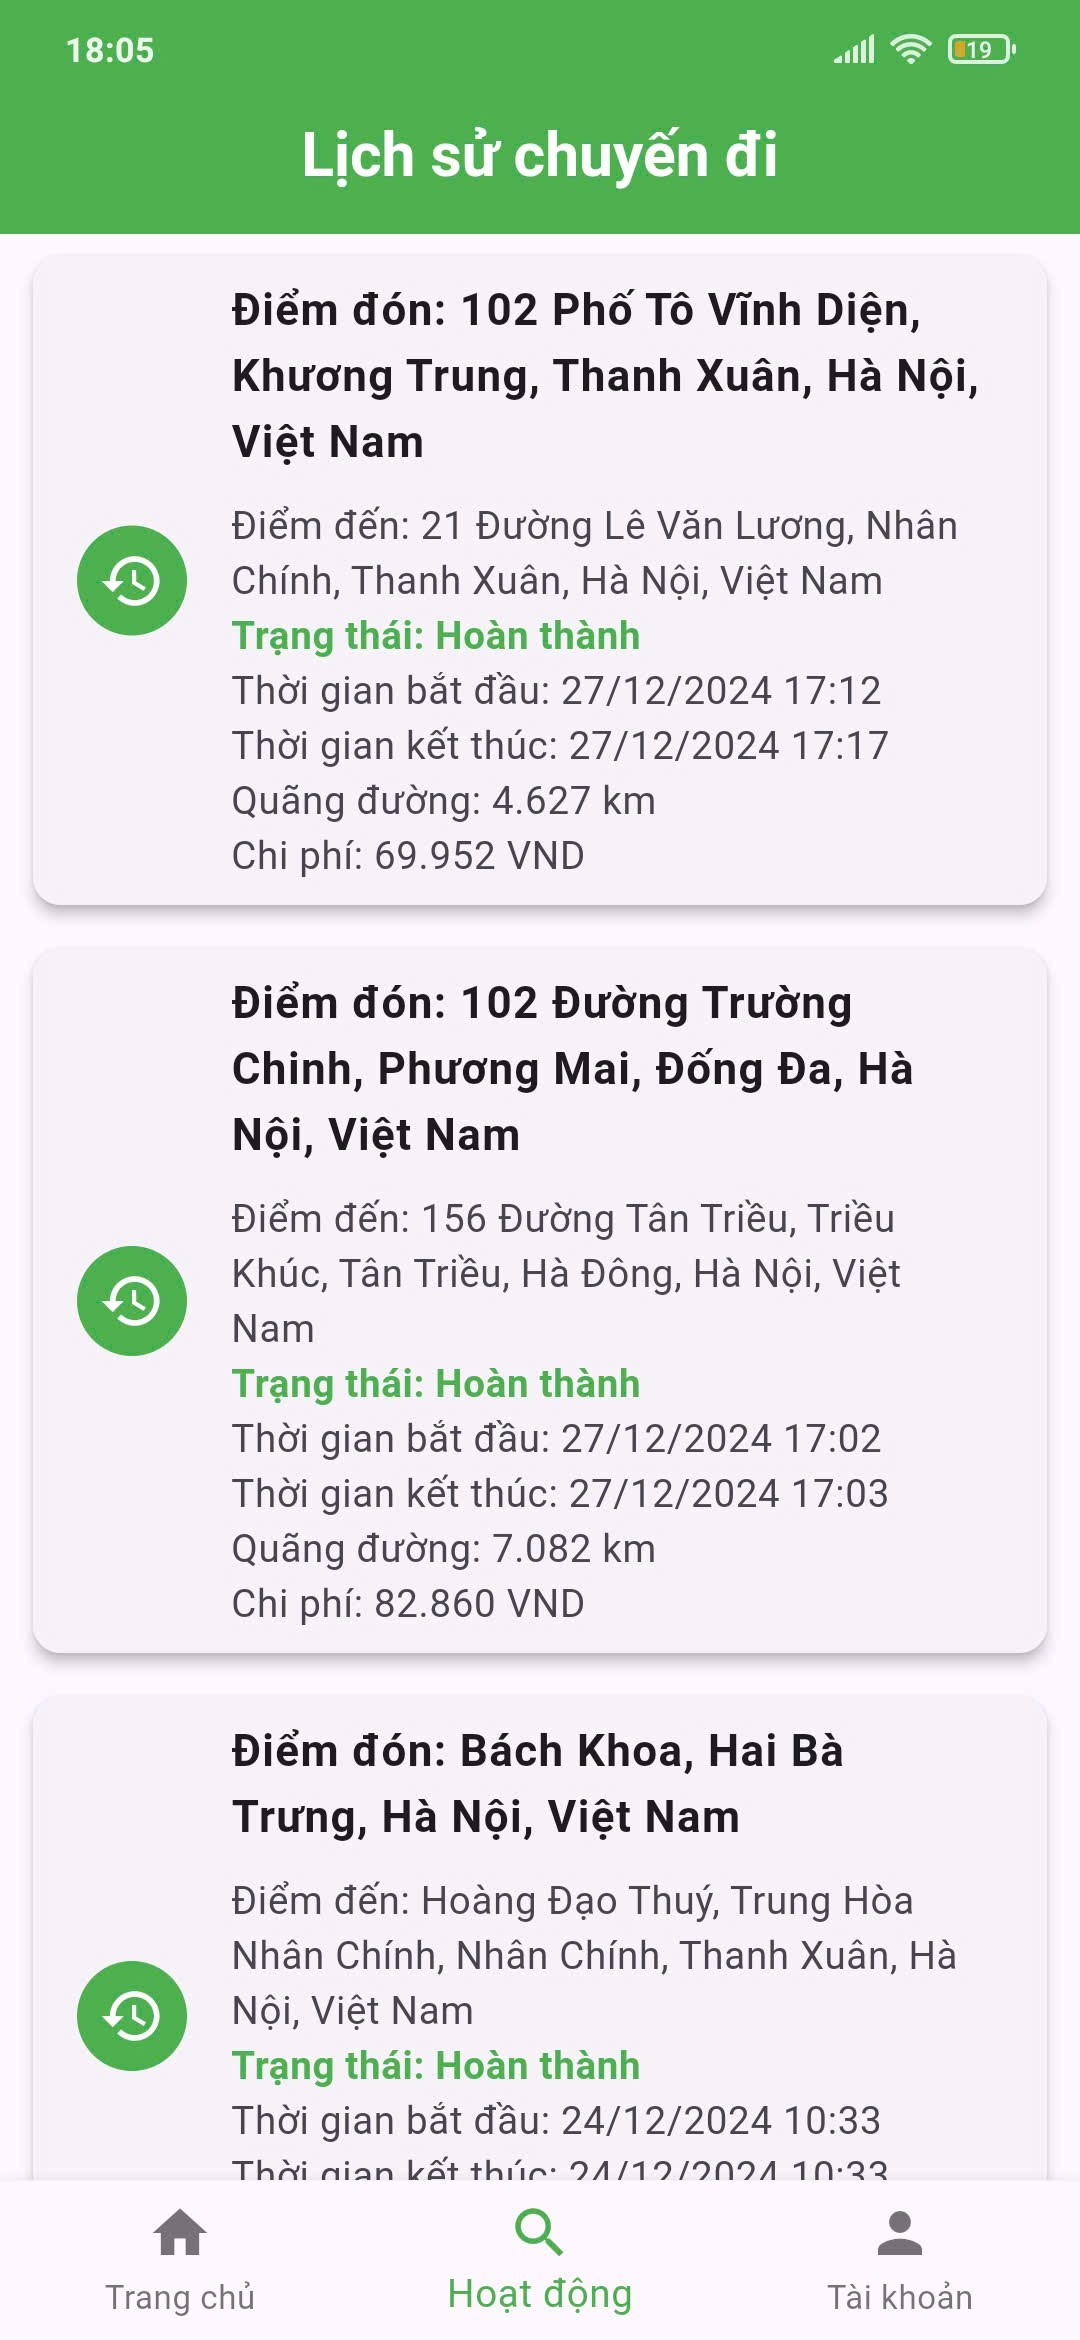
\includegraphics[width=0.8\textwidth]{Hinhve/Lich_su_chuyen_di_nguoi_dung.png}
    \caption{Màn hình Lịch sử chuyến đi của người dùng}
    \label{fig:Lich_su_chuyen_di_nguoi_dung}
\end{figure}

Khi nhấn vào phần hoạt động trên app của người dùng thì phần lịch sử hoạt động này sẽ hiện ra.
Nó cho người dùng biết rằng họ đã thực hiện những chuyến đi nào và thông tin về những chuyến đi đó.

Giao diện màn hình Tài khoản người dùng:
\begin{figure}[H]
    \centering
    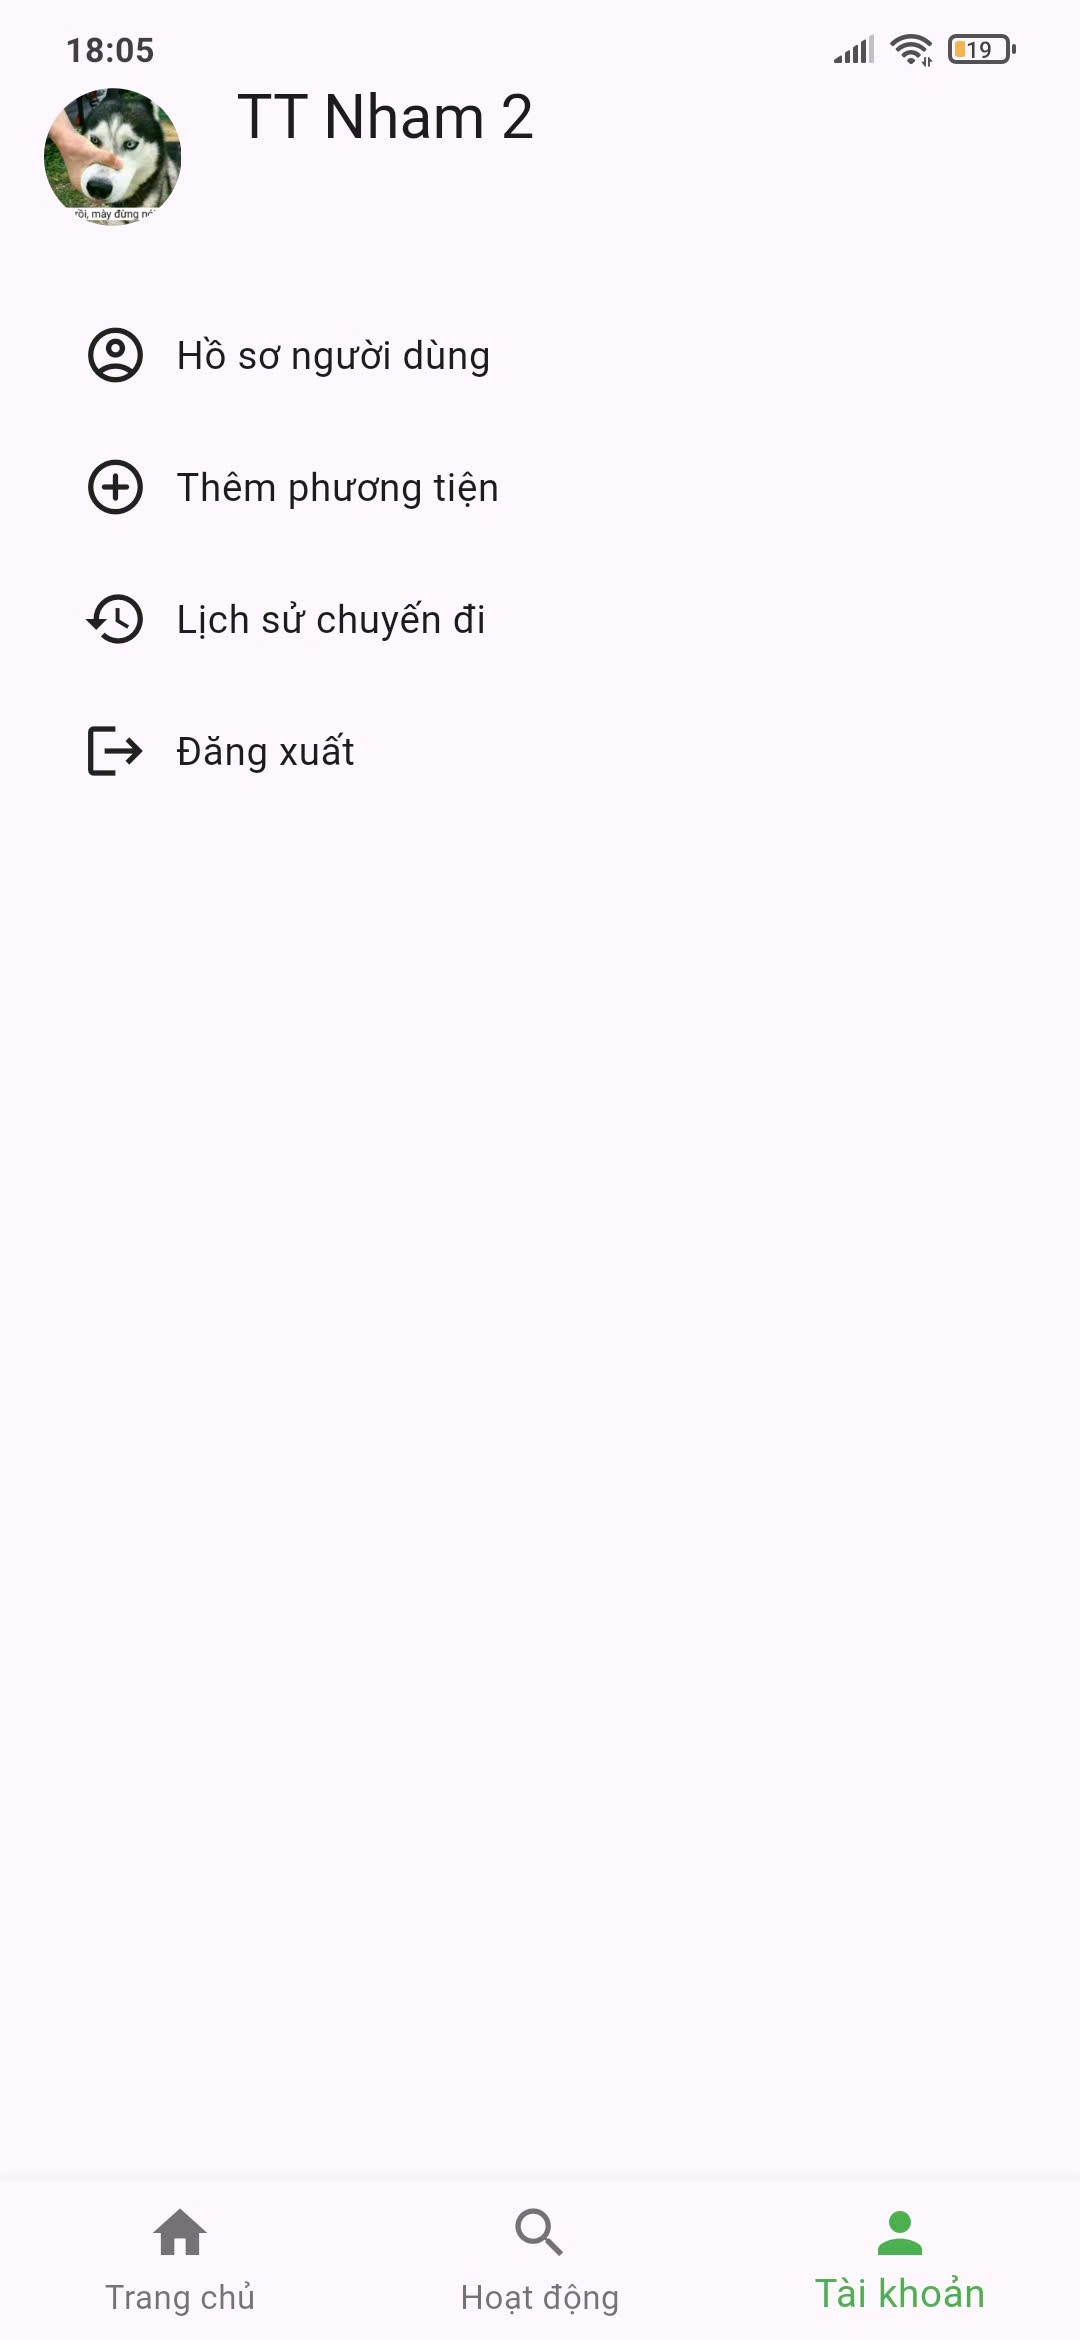
\includegraphics[width=0.8\textwidth]{Hinhve/Tai_khoan_nguoi_dung.png}
    \caption{Màn hình Tài khoản người dùng}
    \label{fig:Tai_khoan_nguoi_dung}
\end{figure}

Sau khi người dùng đăng nhập vào ứng dụng có thể nhấn vào phần "Tài khoản" để xem thông tin về tài khoản của họ.
Người dùng có thể thay đổi thông tin bằng cách nhấn vào phần "Hồ sơ người dùng".
Thêm phương tiện muốn lái hộ bằng cách nhấn vào phần "Thêm phương tiện" hoặc muốn thoát ứng dụng thì nhấn vào phần "Đăng xuất".

Giao diện màn hình Lịch sử chuyến đi của tài xế:
\begin{figure}[H]
    \centering
    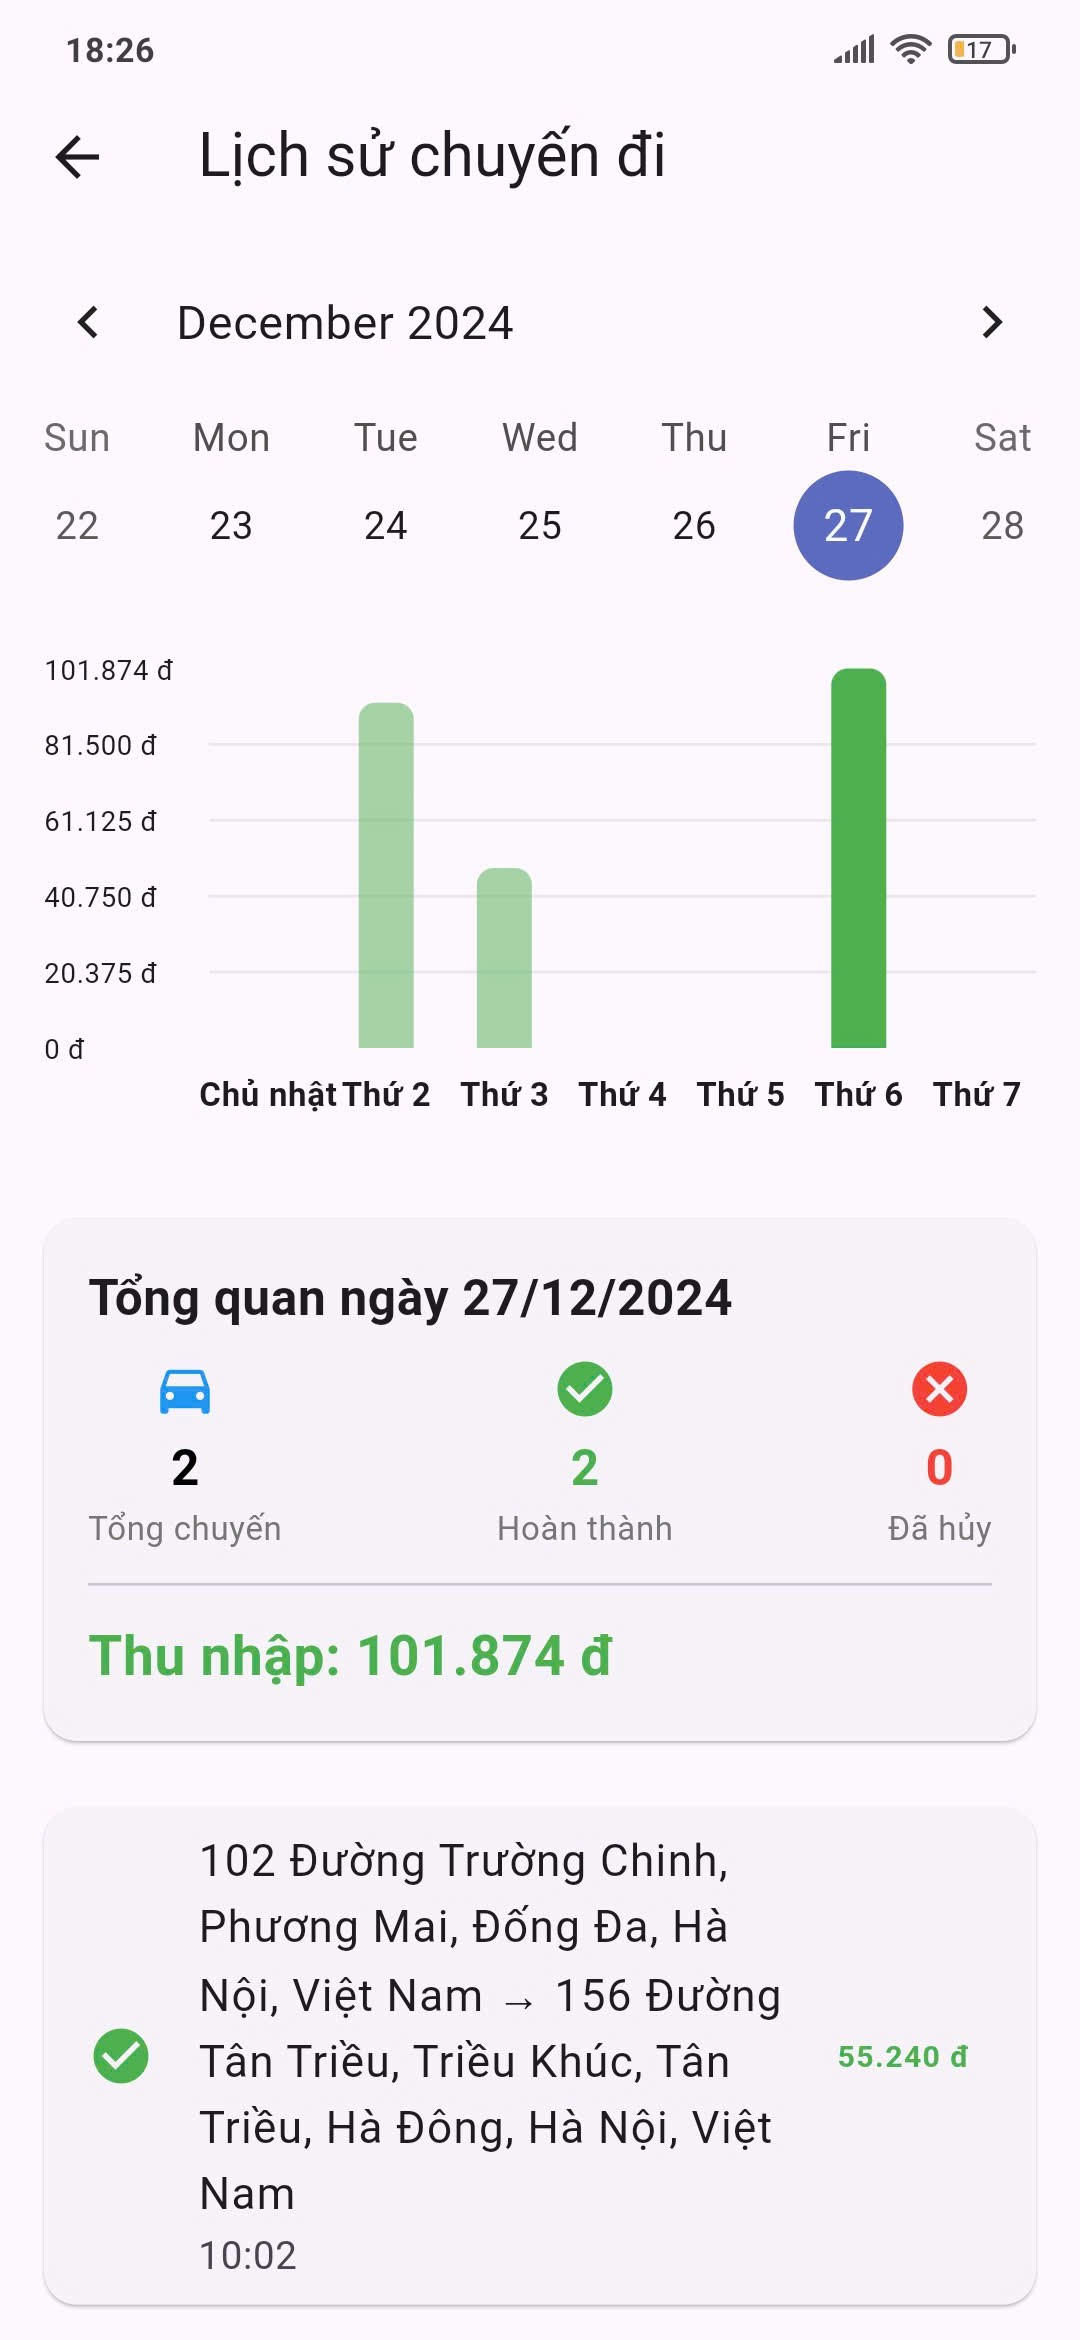
\includegraphics[width=0.8\textwidth]{Hinhve/Lich_su_chuyen_di_driver.png}
    \caption{Màn hình Lịch sử chuyến đi của tài xế}
    \label{fig:Lich_su_chuyen_di_driver}
\end{figure}
Sau khi tài xế đăng nhập, ở màn hình chính, tài xế bấm vào nút đăng nhập để xem thống kê thu nhập và chuyến đi trong ngày.
Thu nhập được thống kê bằng đồ thị theo các ngày trong tuần.
Tài xế có thể thay đổi ngày để xem lịch sử chuyến đi của các ngày khác.

\section{Kiểm thử}
\label{section:4.2}
2-3 trang
2-3 chuc nang

\subsection{Kiểm thử đăng nhập người dùng}
Dữ liệu đầu vào:
\begin{itemize}
    \item phoneNumber: số điện thoại của người dùng.
    \item password: mật khẩu của người dùng.
\end{itemize}
Kết quả trả về:
\begin{itemize}
    \item False: Đăng nhập thất bại, đưa ra lý do đăng nhập thất bại.
    \item True: Đăng nhập thành công, chuyển màn hình sang phần màn hình chính.
\end{itemize}

\begin{table}[H]
    \centering
    \begin{tabular}{|l|l|l|l|}
    \hline
    \textbf{STT} & \textbf{Dữ liệu vào}                          & \textbf{Đầu ra cần đạt}                               & \textbf{Kết quả} \\ \hline
    1            & phoneNumber: null, password:                  & False (Số điện thoại và mật khẩu không được để trống) & Đạt              \\ \hline
    2            & phoneNumber: "", password: "123456"           & False (Số điện thoại không đúng định dạng)            & Đạt              \\ \hline
    3            & phoneNumber: "0123456789", password: ""       & False (Mật khẩu phải có ít nhất 6 ký tự)              & Đạt              \\ \hline
    4 & phoneNumber: "0123456789", password: "000000" & False (Số điện thoại hoặc mật khẩu không chính xác) & Đạt \\ \hline
    5            & phoneNumber: "0372356956", password: "123456" & True (Chuyển sang màn hình chính)                     & Đạt              \\ \hline
    \end{tabular}
\caption{Kiểm thử đăng nhập người dùng}
\label{table:Kiem_thu_dang_nhap_nguoi_dung}
\end{table}

\subsection{Kiểm thử tính chi phí chuyến đi}

Dữ liệu đầu vào:
\begin{itemize}
    \item pickup: tọa độ điểm đón.
    \item destination: tọa độ điểm đến.
\end{itemize}
Kết quả trả về:
\begin{itemize}
    \item False: Đưa ra lý do không tính toán được chi phí.
    \item True: Chuyển sang màn hình đặt xe để xem thông tin.
\end{itemize}

\begin{table}[H]
    \centering
    \begin{tabular}{|l|l|l|l|}
    \hline
    \textbf{STT} & \textbf{Dữ liệu vào}                                                   & \textbf{Đầu ra cần đạt}                         & \textbf{Kết quả} \\ \hline
    1            & pickup: null, destination: null                                        & False(Điểm đến và điểm đón không được để trống) & Đạt              \\ \hline
    2 &
      \begin{tabular}[c]{@{}l@{}}pickup: {latitude: 20.998944,longitude: 105.837814},\\ destination: null\end{tabular} &
      False(Điểm đến và điểm đón không được để trống) &
      Đạt \\ \hline
    3            & pickup: null, \\destination: {latitude: 21.006348,longitude: 105.806999} & False(Điểm đến và điểm đón không được để trống) & Đạt              \\ \hline
    4 &
      \begin{tabular}[c]{@{}l@{}}pickup: {latitude: 20.998944,longitude: 105.837814},\\ destination: {latitude: 21.006348,longitude: 105.806999}\end{tabular} &
      True(Chuyển sang màn đặt tài xế và hiển thị giá tiền chuyến đi) &
      Đạt \\ \hline
    \end{tabular}
    \caption{Kiểm thử tính chi phí chuyến đi}
    \label{table:Kiem_thu_tinh_chi_phi_chuyen_di}
\end{table}

\section{Triển khai}
Sinh viên trình bày mô hình và/hoặc cách thức triển khai thử nghiệm/thực tế. Ứng dụng của sinh viên được triển khai trên server/thiết bị gì, cấu hình như thế nào. Kết quả triển khai thử nghiệm nếu có (số lượng người dùng, số lượng truy cập, thời gian phản hồi, phản hồi người dùng, khả năng chịu tải, các thống kê, v.v.)

Trong dự án này, em đã thực hiện build file apk của ứng dụng ViSafe BK:
\begin{itemize}
    \item Triển khai version 1 với sự trợ giúp của Flutter
    \item Ứng dụng có thể tải từ các thiết bị Android
\end{itemize}
Các bước để kiểm tra ứng dụng trên môi trường máy local:
\begin{itemize}
    \item Bước 1: Cài đặt và cấu hình môi trường cần thiết để chạy thiết bị (Git, NodeJS, Firebase, Flutter).
    \item Bước 2: Tải mã nguồn từ Github hoặc giải nén từ file zip.
    \item Bước 3: Chạy lệnh "npm i" trong thư mục server.
    \item Bước 4: Chạy lệnh "flutter pub get" trong thư mục của ứng dụng user và driver.
    \item Bước 5: Cấu hình biến môi trường cho môi trường server.
    \item Bước 6: Chạy lệnh "npm run start:dev" để chạy server.
    \item Bước 7: Thay đổi đường dẫn của api trong cấu hình ứng dụng driver và user. Nếu chạy trên máy ảo thì dùng "http://10.0.2.2:3000" hoặc dùng máy vật lý thì sẽ dùng địa chỉ ipv4 của máy chạy server.
    \item Bước 8: Dùng lệnh "flutter run" để chạy ứng dụng user và driver.
\end{itemize}
\end{document}
